\section{Тема 13}

\subsection*{Дървета. Индуктивна и неиндуктивна дефиниция на „дърво“. Еквивалентност на тези две дефиниции}

\begin{definition}[не-индуктивна дефиниция]
    Дърво е всеки граф, който е свързан и ацикличен. \\
    \begin{minipage}{0.45\textwidth}
        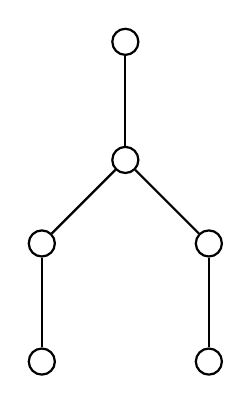
\begin{tikzpicture}[node distance={15mm}, thick, main/.style = {draw, circle}] 
            \node[main] (1) {}; 
            \node[main] (2) [below of=1] {};
            \node[main] (3) [below left of=2] {};
            \node[main] (4) [below right of=2] {}; 
            \node[main] (5) [below of=3] {};
            \node[main] (6) [below of=4] {};
            \draw (1) -- (2);
            \draw (2) -- (3);
            \draw (2) -- (4);
            \draw (3) -- (5);
            \draw (4) -- (6);
        \end{tikzpicture} 
    \end{minipage}
    \hfill
    \begin{minipage}{0.45\textwidth}
        \begin{tikzpicture}
            \node[state] (center) at (0, 0) {};
            \foreach \phi in {1,...,6} {
                \node[state] (v_\phi) at (360/6 * \phi:2cm) {};
                \draw (v_\phi) -- (center);
            }
        \end{tikzpicture}
    \end{minipage}
\end{definition}

\begin{definition}[индуктивна дефиниция]
    Множеството от дърветата се дефинира така: \\
    \bu{База}: всеки тривиален граф е дърво \\
    \bu{Индуктивна стъпка}: ако \mexpr{T = (V, E)} е дърво и u е връх в T и w е връх, който не е в T, то 
    \mexpr{T' = (V \cup \{w\}, \{(u, w)\} \cup E)} е дърво.
\end{definition}

\begin{lemma}
    Индуктивна и не-индуктивна дефиниция са еквивалентни.
\end{lemma}

\begin{proof}
    \(\newline\text{I)}\) Ще докажем, че всеки граф, генериран от индуктивната дефиниция, е свързан и 
    ацикличен. \\
    \bu{База:} разглеждаме граф \((\{u\}, \emptyset)\), който очевидно е свързан и ацикличен. \\
    \bu{Индукционно предположение:} допускаме, че \mexpr{T = (V, E)} от индуктивната стъпка е свързан и ацикличен. \\
    \bu{Индукционна стъпка:} за да бъде свързан, трябва за всеки два върха \(x, y \in V(T')\) да е изпълнено, че
    има път между тях. Но \mexpr{V(T') = V \cup \{w\}}, тогава:
    \begin{itemize}
        \item нито един от x, y не е връх от w. Но тогава е вярно, че \mexpr{x, y \in V}. Съгласно 
        индуктивното предположение, между всеки два върха в T има път, от което следва, че в T' има път 
        между всеки два върха от V
        \item точно единият от x и y е връх w. Б.О.О., нека това е връх x. Тогава задължително \(y \in V\).
        Но тогава и y, и w са върхове в T. Съгласно И.П., в T има път p между тях. Тогава p е път между y и 
        u в T', от което следва, че при слепването на p, реброто (u, w) и върха w се получава път между y и
        x = w в T'.
        \item x = y = w. Тогава между x и y има тривиален път с дължина 0. 
    \end{itemize}
    Така доказахме, че \(T'\) е свързан. \\
    Нито един връх от \(T'\) не може да участва в цикъл, понеже:
    \begin{itemize}
        \item връх w е от степен 1, а всеки връх, който е в цикъл, е от степен поне 2
        \item останалите върхове на \(T'\) са върховете на \(T\), а съгласно И.П. \(T\) е ацикличен и добавянето на 
        реброто \((u, w)\) не може да създаде цикъл от върховете на \(V(T)\).
    \end{itemize}
    Така доказахме, че \(T'\) е свързан. \\
    Следователно \(T'\) е дърво.
    \(\newline\text{II)}\) Ще докажем, че всяко дърво може да бъде коструирано от процедурата на 
    индуктивната дефиниция. \\
    Нека \(D\) е произволно дърво съгласно неиндуктивната дефиниция. \\
    Ако \(D\) има точно един връх, то \(D\) е може да бъде коструирано от базата на индуктивната дефиниция. В 
    противен случай, в \(D\) има поне един висящ връх \(u_1\). \\
    Нека \mexpr{D_1 = D - u_1}. Ако \(D_1\) има точно един висящ връх, то \(D_1\) може да бъде коструирано 
    от базата на индуктивната дефиниция. В противен случай, в \(D_1\) има поне един висящ връх \(u_2\). \\
    Нека \mexpr{D_2 = D_1 - u_2}. Ако \(D_2\) има точно един връх, то \(D_2\) може да бъде коструирано от
    базата на индуктивната дефиниция. И т.н. \\
    При всяко от изтриванията на висящ връх, графът остава свързан и ацикличен, тоест дърво. Следователно 
    има редица от дървета \mexpr{D, D_1, D_2}, ..., \(D_k\) за някое \(k\). Последователното изтриване на 
    върхове може да се направи само краен брой пъти, защото началното дърво \(D\) има краен брой върхове. 
    И така за някое \(k\) е вярно, че \(D\) има точно един връх. Изтритите върхове са \mexpr{u_1, ..., u_k} в 
    реда на триенето. Тогава графът с точно един връх \(D_k\) може да бъде коструирано от базата на 
    индуктивната дефиниция, а след това \mexpr{|V(D)| - 1} пъти добавяме изтритите върхове в обратния ред 
    на изтриването им, като свързваме всеки от тях към точно този връх, който е бил единственият му съсед 
    точно преди изтриването. Така получаваме началното дърво \(D\). 
\end{proof}

\subsection*{Теореми за: връзката между броя на ребрата и на върховете и за единственост на път между два върха в дърво}

\begin{theorem}[за единственост на път между два върха]
    Граф е дърво \totw между всеки два върха има точно един път.
\end{theorem}
\begin{proof}
    \(\newline\Rightarrow)\) Да разглеждаме произволно дърво \(T\) и произволни \(u, v \in V(T)\). Ще 
    докажем, че има точно един път \(u-v\) път. \\
    От свързаността на \(T\) следва, че има \(u-v\) път, а от това, че е ацикличен следва, че няма повече 
    от един \(u-v\) път. \\
    Да допуснем, че между \(u\) и \(v\) има поне два пътя \(p\) и \(q\). Връх \(u\) се явява край и на \(p\), 
    и на \(q\). Разглеждаме \(p\) и \(q\) като крайни редици от върхове, като търсим първия връх от \(u\) 
    нататък, който е различен за \(p\) и \(q\). Такъв трябва да има, иначе \(p\) и \(q\) биха били един 
    и същи път. Б.О.О., нека \(w\) е първият връх от \(u\) нататък в \(p\), който не се среща в \(q\). 
    Нека \(a\) е върхът преди \(w\) в посока от \(u\) нататък в \(p\), тоест \(a\) е последният от 
    \(u\) нататък в \(p\), който е общ за \(p\) и \(q\). Нека \(b\) е първият връх след \(a\) в \(p\) в 
    посока от \(u\) нататък, който е връх и в \(q\). Такъв общ връх трябва да има, понеже \(p\) и \(q\) 
    имат друг (освен \(u\)) общ край, а именно връх \(v\), така че няма как след \(a\), в посока от 
    \(u\) нататък, да имат само върхове, които не са общи. Така в \(p\) има подпът \(p'\) с краища 
    \(a\) и \(b\), който не е подпът на \(q\). Аналогично, в \(q\) има подпът \(q'\) с краища \(a\) и \(b\), 
    който не е подпът на \(p\). Единият от \(p'\) и \(q'\) може да няма вътрешни върхове, но това няма 
    значение. Тогава \(p' \cup q'\) е цикъл в \(T\), а в дърветата няма цикли. \\
    Следователно, допускането, че има поне два различни \(u-v\) пътя, е грешно.
    \(\newline\Rightarrow)\) Да разглеждаме произволен граф \(G\), в който между всеки два върха има точно 
    един път. Оттук следва, че \(G\) е свързан. \\
    Ако допуснем, че в \(G\) ива поне един цикъл следва, че в \(G\) има поне два върха, между които има два
    различни пътя, което е невъзвожно спрямо направеното допускане, че между всеки два върха има точни 
    един път. \\
    Тогава допускането, че в \(G\) съществува цикъл е погрешно. Следователно \(G\) е ацикличен, а оттам и 
    дърво.
\end{proof}

\begin{theorem}[за връзката между броя на ребрата и на върховете]
    Във всяко дърво е изпълнено, че \(m = n - 1\). (\(n\) - брой върхове, \(m\) - брой ребра).
\end{theorem}
\begin{proof}
    (със структурна индукция) \\
    \bu{База:} разглеждаме граф само с един връх (\(n = 1\)) без ребра (\(m = 0\)).
    \bu{Индукционно предположение:} нека твърдението е изпълнено за дървото \(T\), т.е. 
    \mexpr{|E(T)| = |V(T)| - 1} \\
    \bu{Индукционна стъпка:} ще докажем твърдението за дървото \(T'\), т.е. \mexpr{|E(T')| = |V(T')| - 1}. \\
    Имаме, че \mexpr{|E(T') = |E(T)| + 1} и \mexpr{|V(T') = |V(T)| + 1}, откъдето получаваме, че 
    \mexpr{|E(T)| + 1 = |V(T)| + 1 - 1 \implies |E(T)| = |V(T)| - 1}, което е точно изпълнено за дървото \(T\)
    от И.П.
\end{proof}

\subsection*{Коренови дървета. Височина и разклоненост на кореновите дървета. Представяния на дървета}



\subsection*{Покриващо дърво. Теорема за съществуване на покриващо дърво}
\begin{definition}
    Нека \graf е свързан граф. Покриващо дърво на \(G\) е всяко дърво \(T = (V, E')\), където \(E' \subseteq E\).
\end{definition}

\begin{theorem}
    За всеки граф \graf има поне едно покриващо дърво \totw \(G\) е свързан.
\end{theorem}
\begin{proof}
    \(\newline\Rightarrow)\) Ако \(G\) има покриващо дърво, то \(G\) е свързан, понеже между всеки два 
    върха има път, което влече съществуване на път между тези два върха на \(G\).
    \(\newline\Leftarrow)\) Ако \(G\) е свързан, то следният алгоритъм строи покриващо дърво на \(G\): \\
    Вход: свързан граф \mexpr{G = (\{v_1, ..., v_n\}, E)} \\
    Изход: покриващо дърво на \(G\)
    \begin{enumerate}
        \item Ако \(G\) няма цикли, върни \(G\) и край
        \item В противен случай, нека \(c\) е произволен цикъл в \(G\) и \(e\) е произволно ръбро от \(c\)
        \item Правим \(G \leftarrow G - e\) и отиваме на 1) 
    \end{enumerate}
    (Д-во за коректност?)
\end{proof}